\chapter{Nanowire Structure and Measurement}
In this chapter, we present the experiment data and some analysis which are the foundation of our circuit design.
The first section describes briefly the silicon nanowire in our experiments.
The second section analyzes the data of the biology experiments.
The third section presents the data of the electrical measurement.
The last section provides the design specification based on the information given by the previous sections.

\section{Brief Description of Nanowire Structure}
The nanowire we use is made by Prof.Yang's team (National Chiao Tong University)\cite{C5}.
Fig.\ref{fig:drawing} is the cross-sectional view of the nanowire structure.
The fabrication process is based on the poly-silicon sidewall spacer technique.
The n-Type doped poly-SiNW FET has two to ten poly-silicon channels.
Each channel is 80nm in width and 2µm in length.
A Large portion of the channel surface is exposed to the environment.
The exposed region, through several post-process steps, captures the DNA probe and serves as the sensing site for DNA molecules.\cite{C5, C6}


\begin{figure}[!htbp]
    \centering
    \begin{minipage}[t]{0.4\textwidth}
        \includegraphics[width=1\linewidth]{images/chapter3/Nw.png}
        \raggedleft
        (a)
    \end{minipage}
    \hfill
    \begin{minipage}[t]{0.4\textwidth}
        \includegraphics[width=1\linewidth]{images/chapter3/Nw_section.png}
        \raggedleft
        (b)
    \end{minipage}
    \caption{Nanowire Structure.  \textbf{(a)} A nanowire device with two poly-silicon channels. \textbf{(b)} The sectional view of the cutting plane in (a). }
    \label{fig:drawing}
\end{figure}


\section{Biology Experiment}
The biology experiment data are provided by Prof.Yang's team.
These data are the Id-Vg measurement of the same biomolecule placed under different circumstances or with different nanowire devices.
With each measurement repeated for three times, we find the mean and standard deviation (SD) of them and consider the SD value as the intrinsic noise of nanowire.
We want to ensure that such noise should not be greater than the signal.
To be more specific, we examine whether the Id-Vg curves of different concentrations overlap with others or not.
An example is presented below:
\begin{figure}[!htb]
    \centering
    \begin{minipage}[t]{1\textwidth}
        \centering
        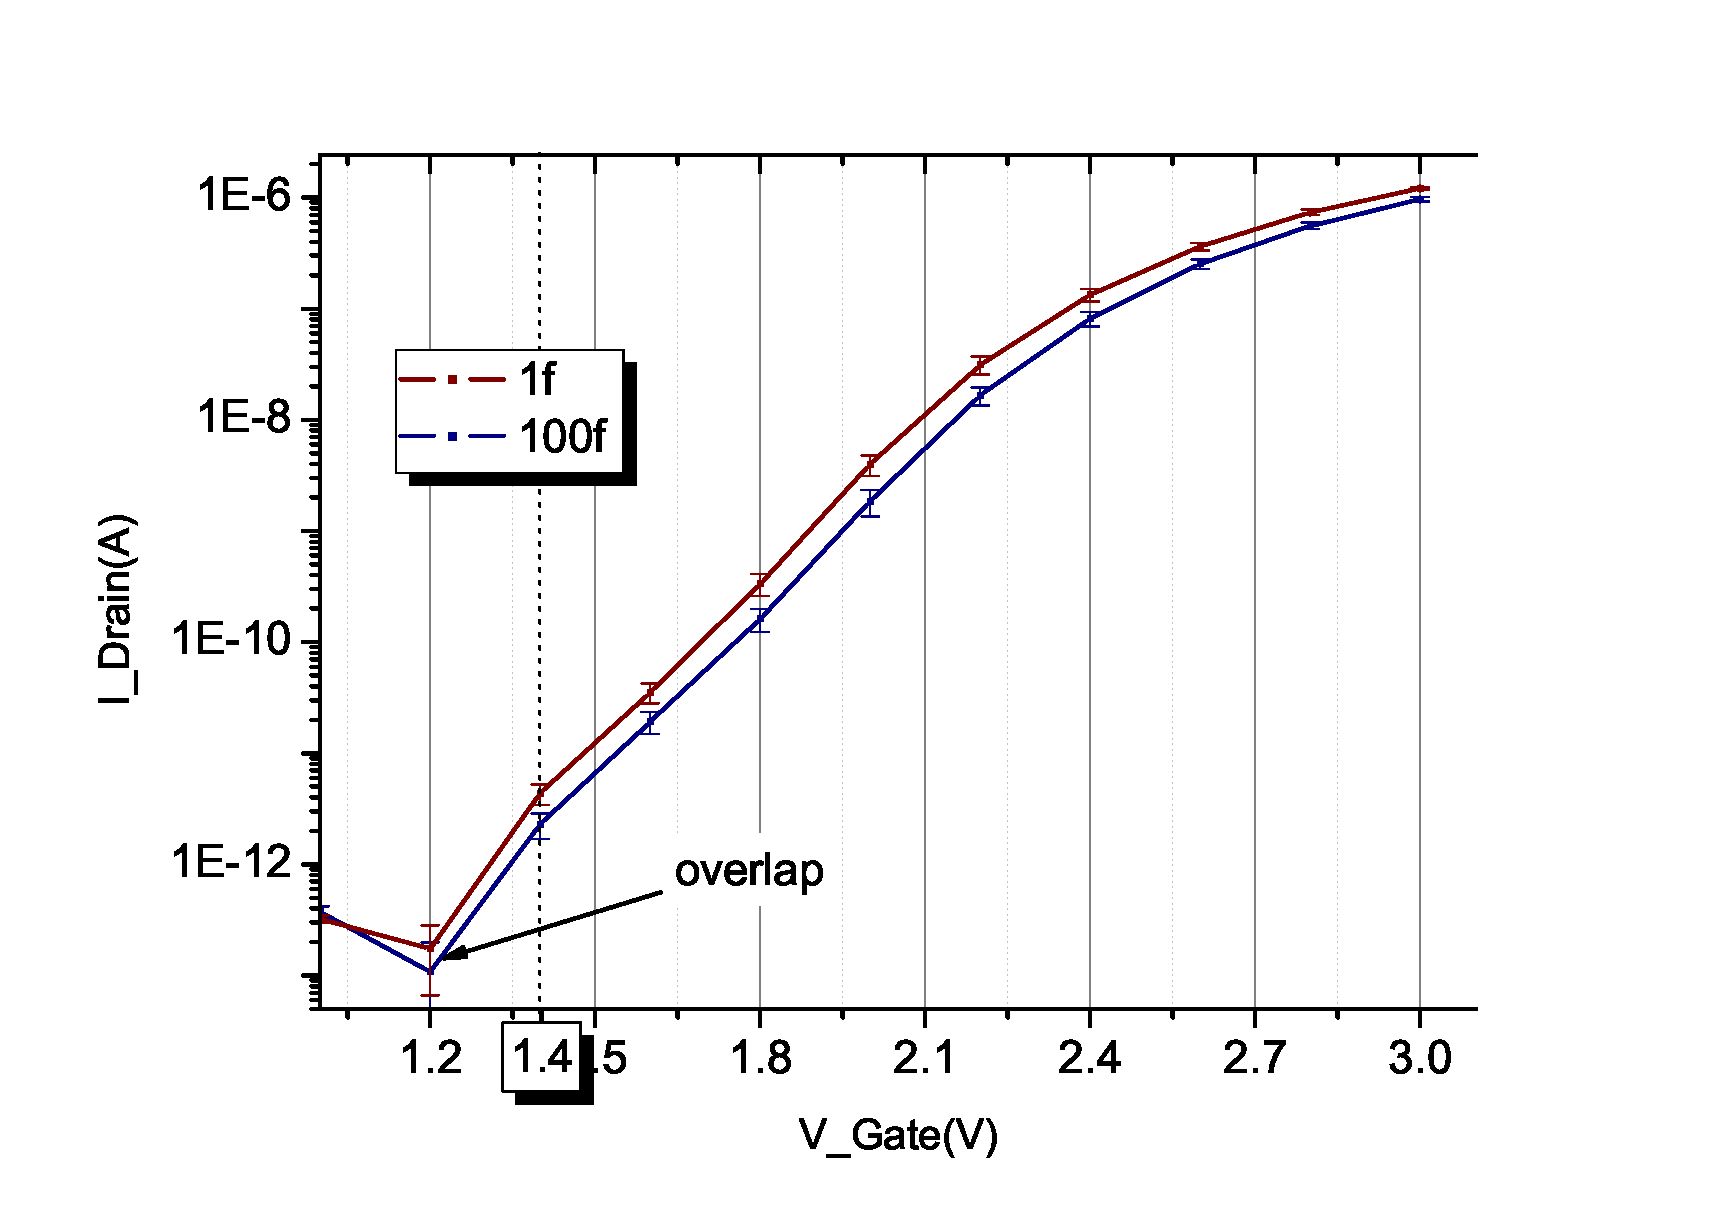
\includegraphics[scale=0.4]{images/chapter3/208_devices/L2-8_log.eps}
        (a)
    \end{minipage}
    \vfill
    \begin{minipage}[t]{1\textwidth}
        \centering
        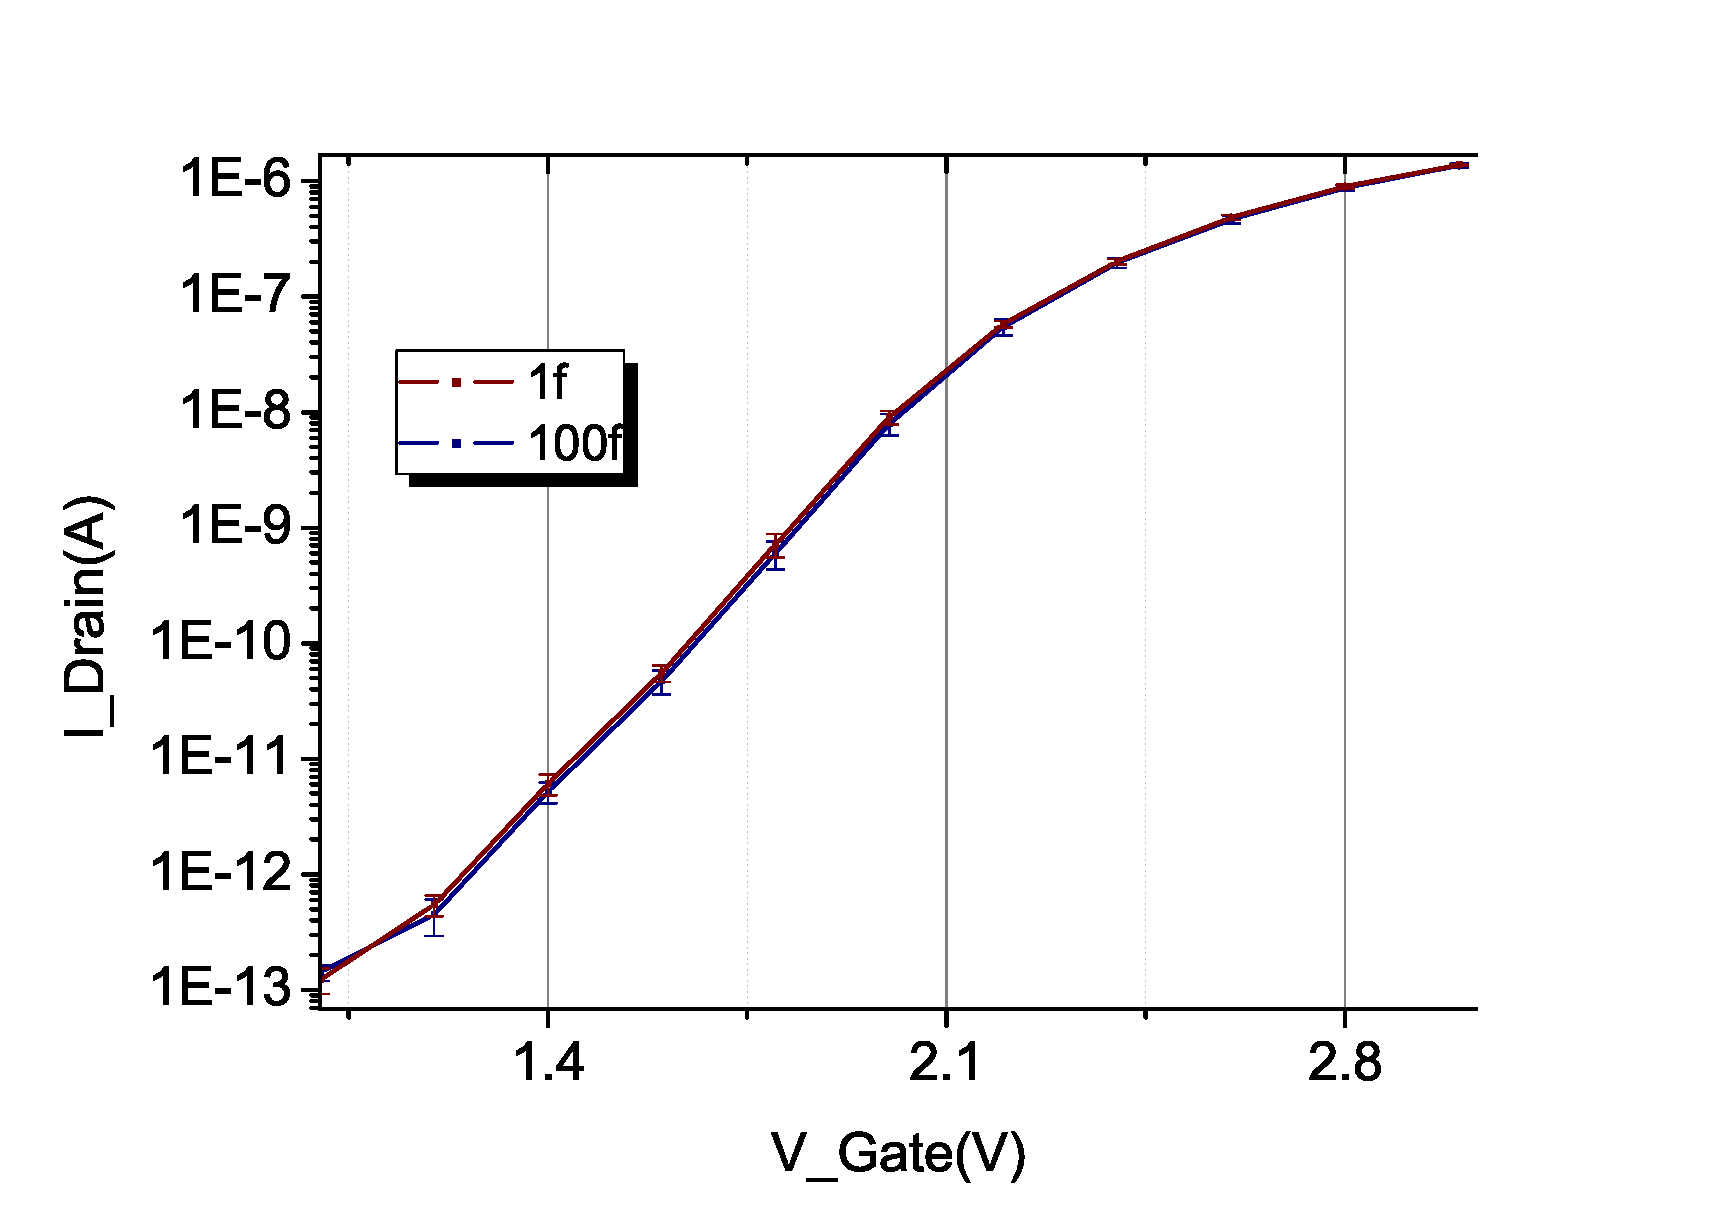
\includegraphics[scale=0.4]{images/chapter3/208_devices/L2-10_log.eps}
        (b)
    \end{minipage}
    \caption{Concentration-dependent $I_D$-$V_G$ curves of two equivalent nanowire devices.
    In \textbf{(a)}, the measurement result of 1fM and 100fM biomolecule solution is distinguishable. There is no overlap between two curves. This is not true in \textbf{(b)}.}
    \label{fig:SD_sucandfail}
\end{figure}

Fig.\ref{fig:SD_sucandfail} are concentration-dependent measurements (1 femto mole(fM) and 100fM biomolecule solution) obtained with two devices ((a) and (b)).
The two curves in (a) are distinguishable from each other after gate voltage is above 1.4v.
They are not distinguishable in (b) since they overlap with each other.
We thus assert that the device of (b) can not detect the concentration difference between 1fM and 100fM.
The noise is stronger than the signal (The signal means difference in $I_D$ caused by the concentration difference).
The device of (a) can do so if it is biased at a gate voltage larger than 1.4v or a drain current larger than 1E-11.

\begin{figure}[!htb]
        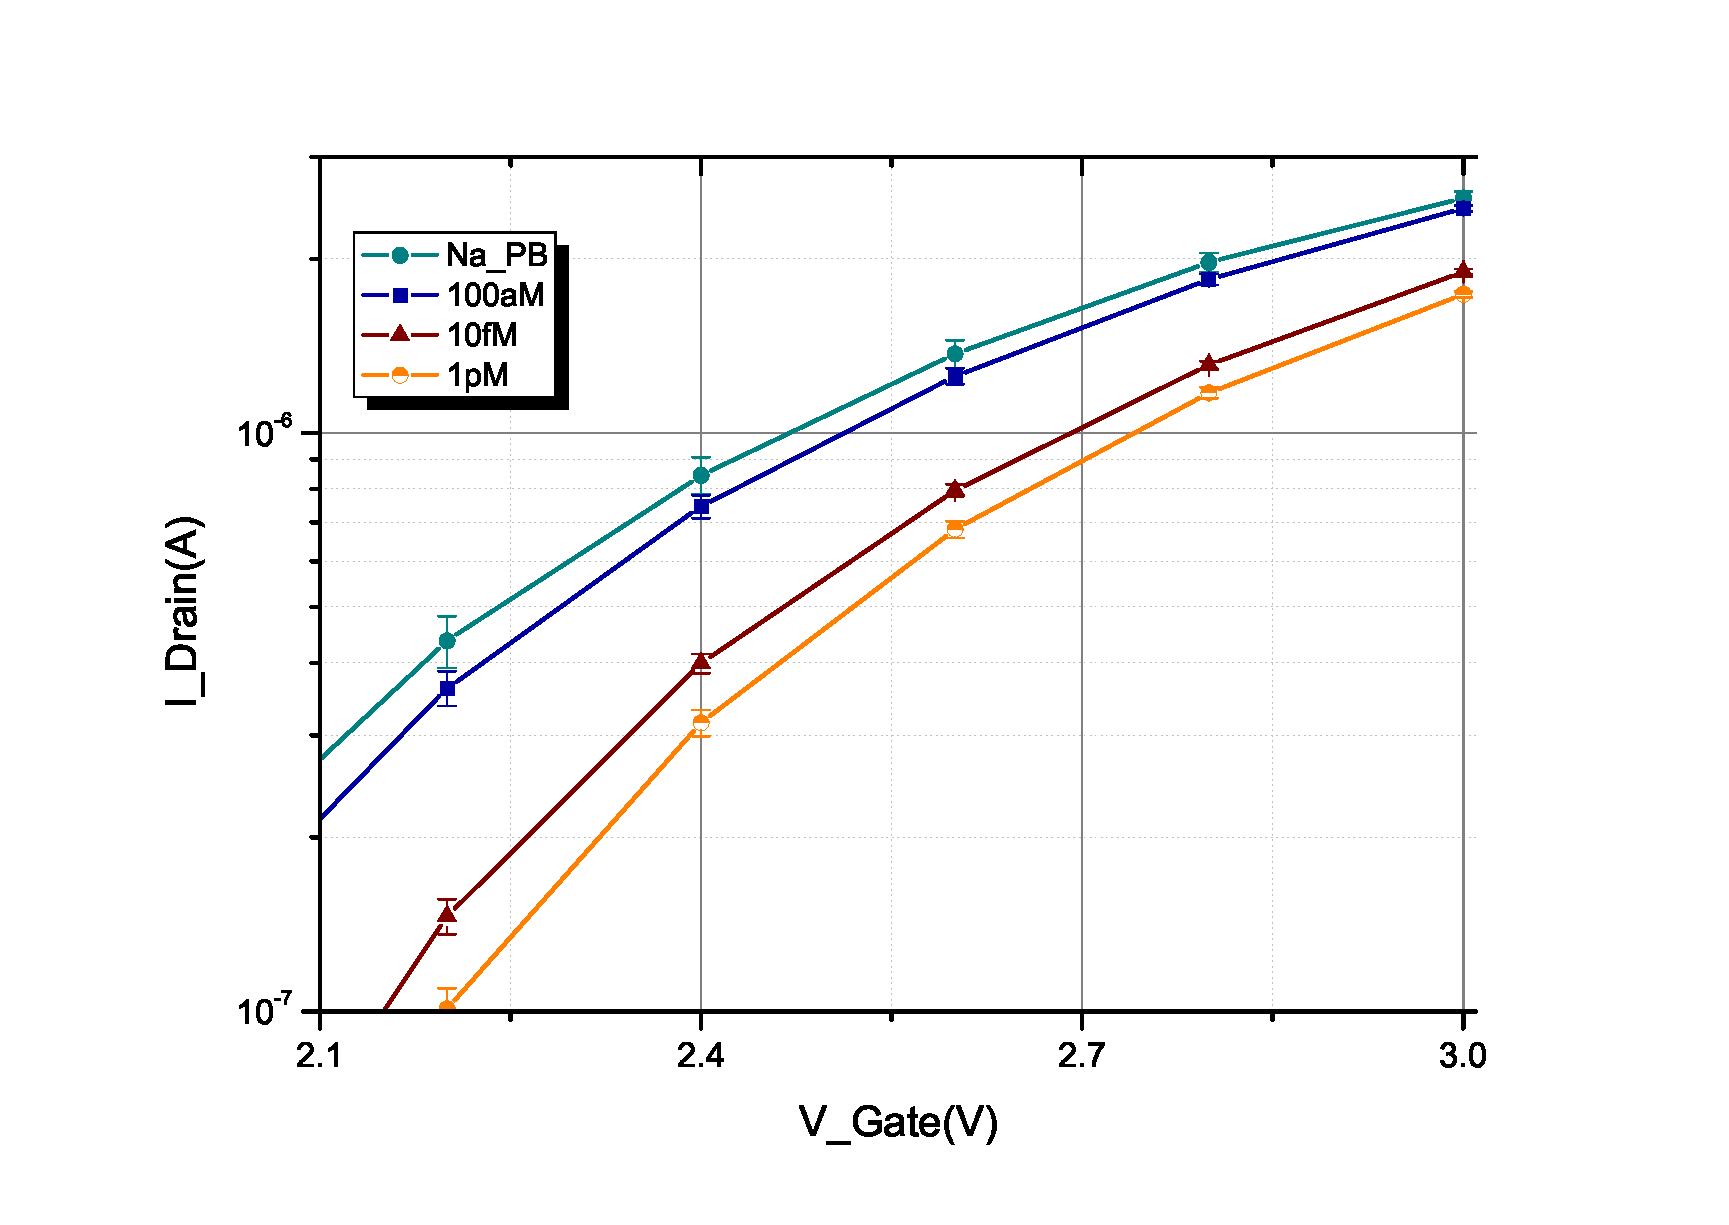
\includegraphics[width=1\textwidth]{images/chapter3/128_allT_mag.eps}
    \caption{Concentration-dependent $I_D$-$V_G$ curves with concentration of Na\_PB(Buffer solution only), 100aM, 10pM, 1pM.
    Since the biomolecule is negative-charged, the lower the concentration is, the higher the curve is.
    To be noticed, the 10fM curve is closer to the curve of 1pM than 100aM.
     }
    \label{fig:SD_allT}
\end{figure}

In Fig.\ref{fig:SD_allT}, $I_D$ increases with the biomolecule concentration.
One can find that there is only a small separation between the curve for PBS buffer and the solution containing 100aM of biomolecules.
Hence 100aM should be the limit of detection.

It is worth noting that there is more significant difference between the curves for 100aM and 10fM than that between 10fM and 1pM.
Besides, Fig.\ref{fig:SD_allT2} shows that the normalized variation: ${SD} / {Mean}$ has not much to do with concentration.
Hence, the analysis indicates that the ``resolution'' for detecting concentration ranging from 100aM to 10fM may be better than the that ranging from 10fM to 1pM.
\begin{figure}[tb]
    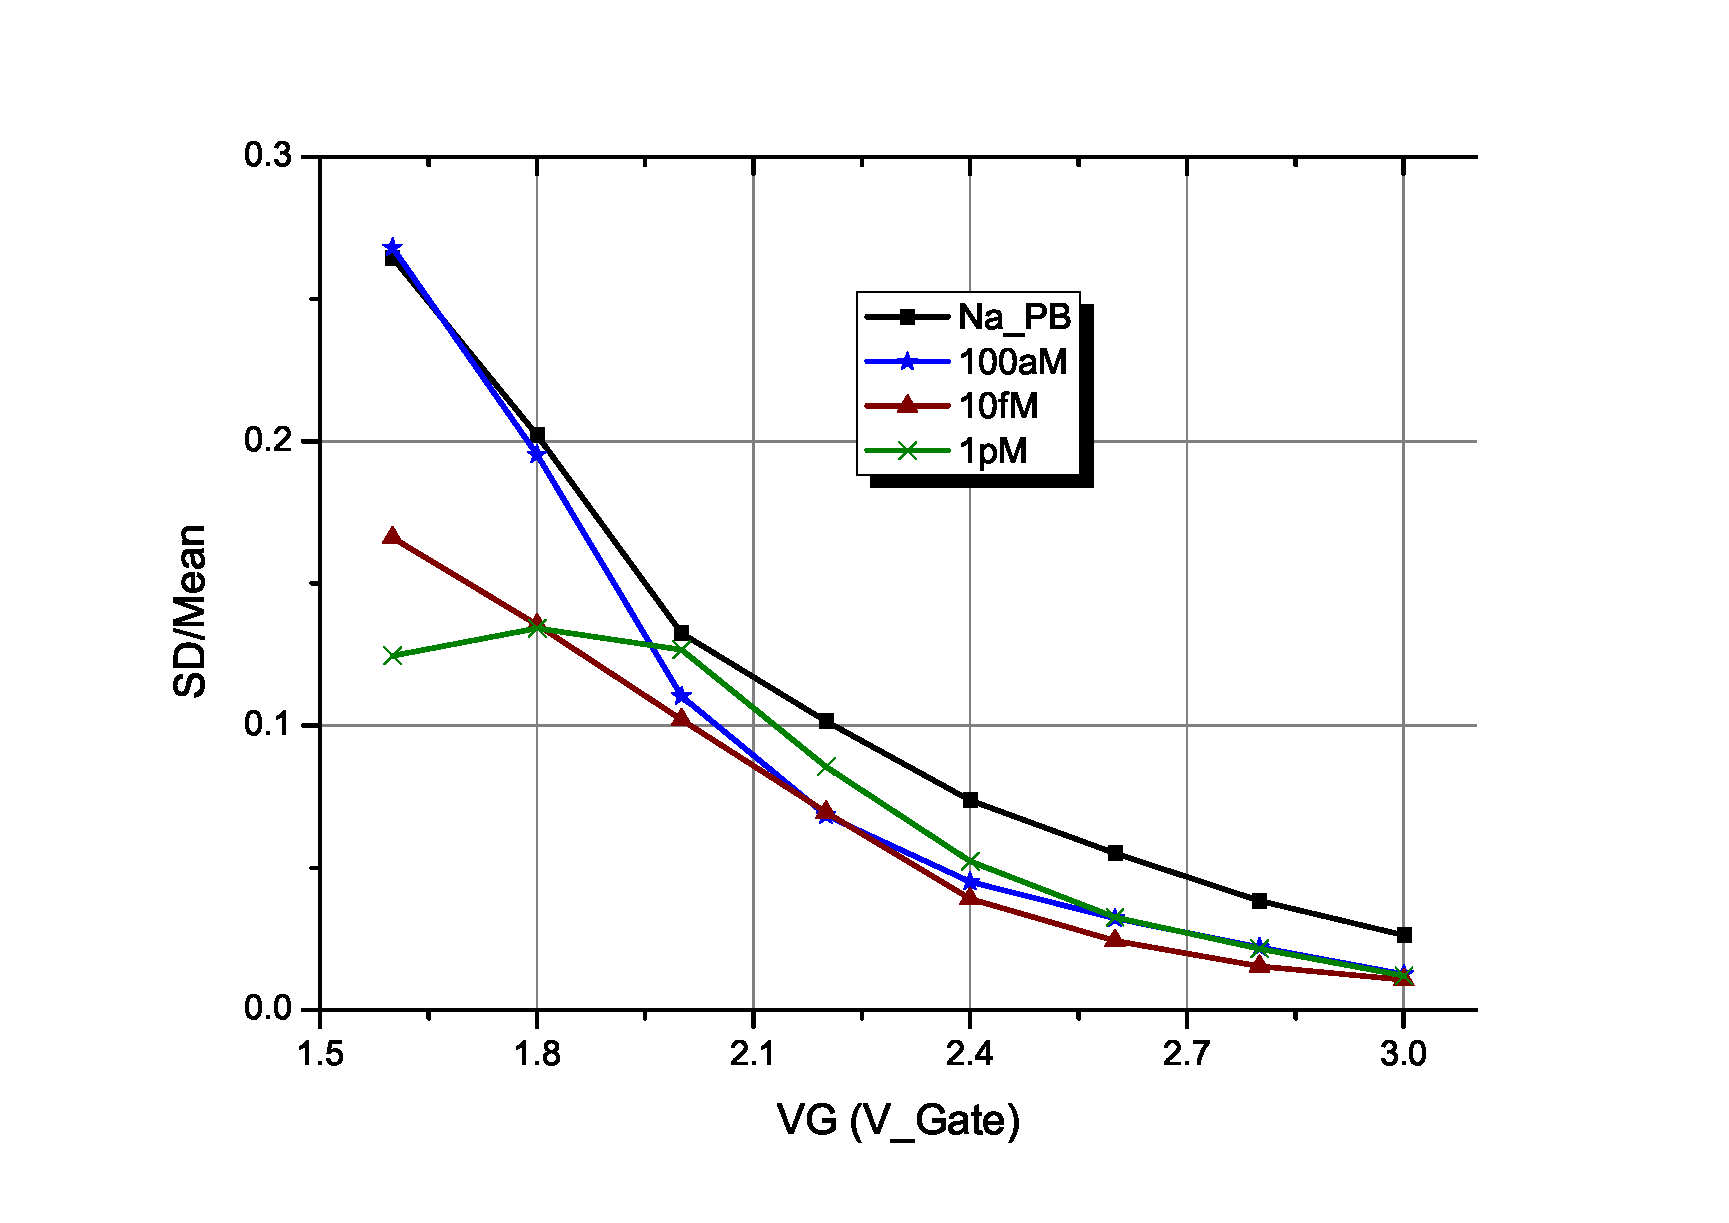
\includegraphics[width=1\textwidth]{images/chapter3/128_allT_error.eps}
    \caption{The normalized variation of Fig.\ref{fig:SD_allT}. The normalized variation is obtained by dividing SD by Mean.}
    \label{fig:SD_allT2}
\end{figure}

\subsection{Appropriate operation region} \label{section:biasVg}
In \cite{C6}, the team found that the current change ($I_D$) induced by biomolecules was dependent on the applied gate voltage (VG).
A device with a larger $I_D$ change means that the device is more sensitive to the concentration difference.
Thus, the team tried to find a biasing gate voltage which concentration difference can induce more $I_D$ change.

We also want to operate the nanowire under the condition that the device has higher sensitivity.
Differently, we suppose that one should find the appropriate operation region instead of a bias range for $V_G$.
We also take noise into consideration.
The comprehensive method we proposed below proves that the nanowire should be operated in the weak inversion region adjacent to the transition region.

Our method is that we choose the operation region with more ``noise tolerance''.
The noise tolerance is defined as below:
\setlength{\mathindent}{2cm}
\begin{align}
    \text{For} \quad & I_{D1} > I_{D2} \\
    & \text{Noise Tolerance} = \frac{\text{Noiase Margin}}{I_{D2}} \\
    & \text{Noise Margin} = (I_{D1} - S_{D1}) - (I_{D2} + S_{D2})
\end{align}
$I_D$ and $SD$ are the mean and standard deviation of several $I_D$-$V_G$ curves obtained in a same experimental condition.
The larger the noise tolerance implies there is more space between two curves.
And more space implies the less chance of overlapping that may happen between two concentration curves.


\begin{figure}[!hbt]
    \centering
    \begin{minipage}[t][20cm][t]{1\textwidth}
        \begin{minipage}[t]{0.5\textwidth}
            \centering
            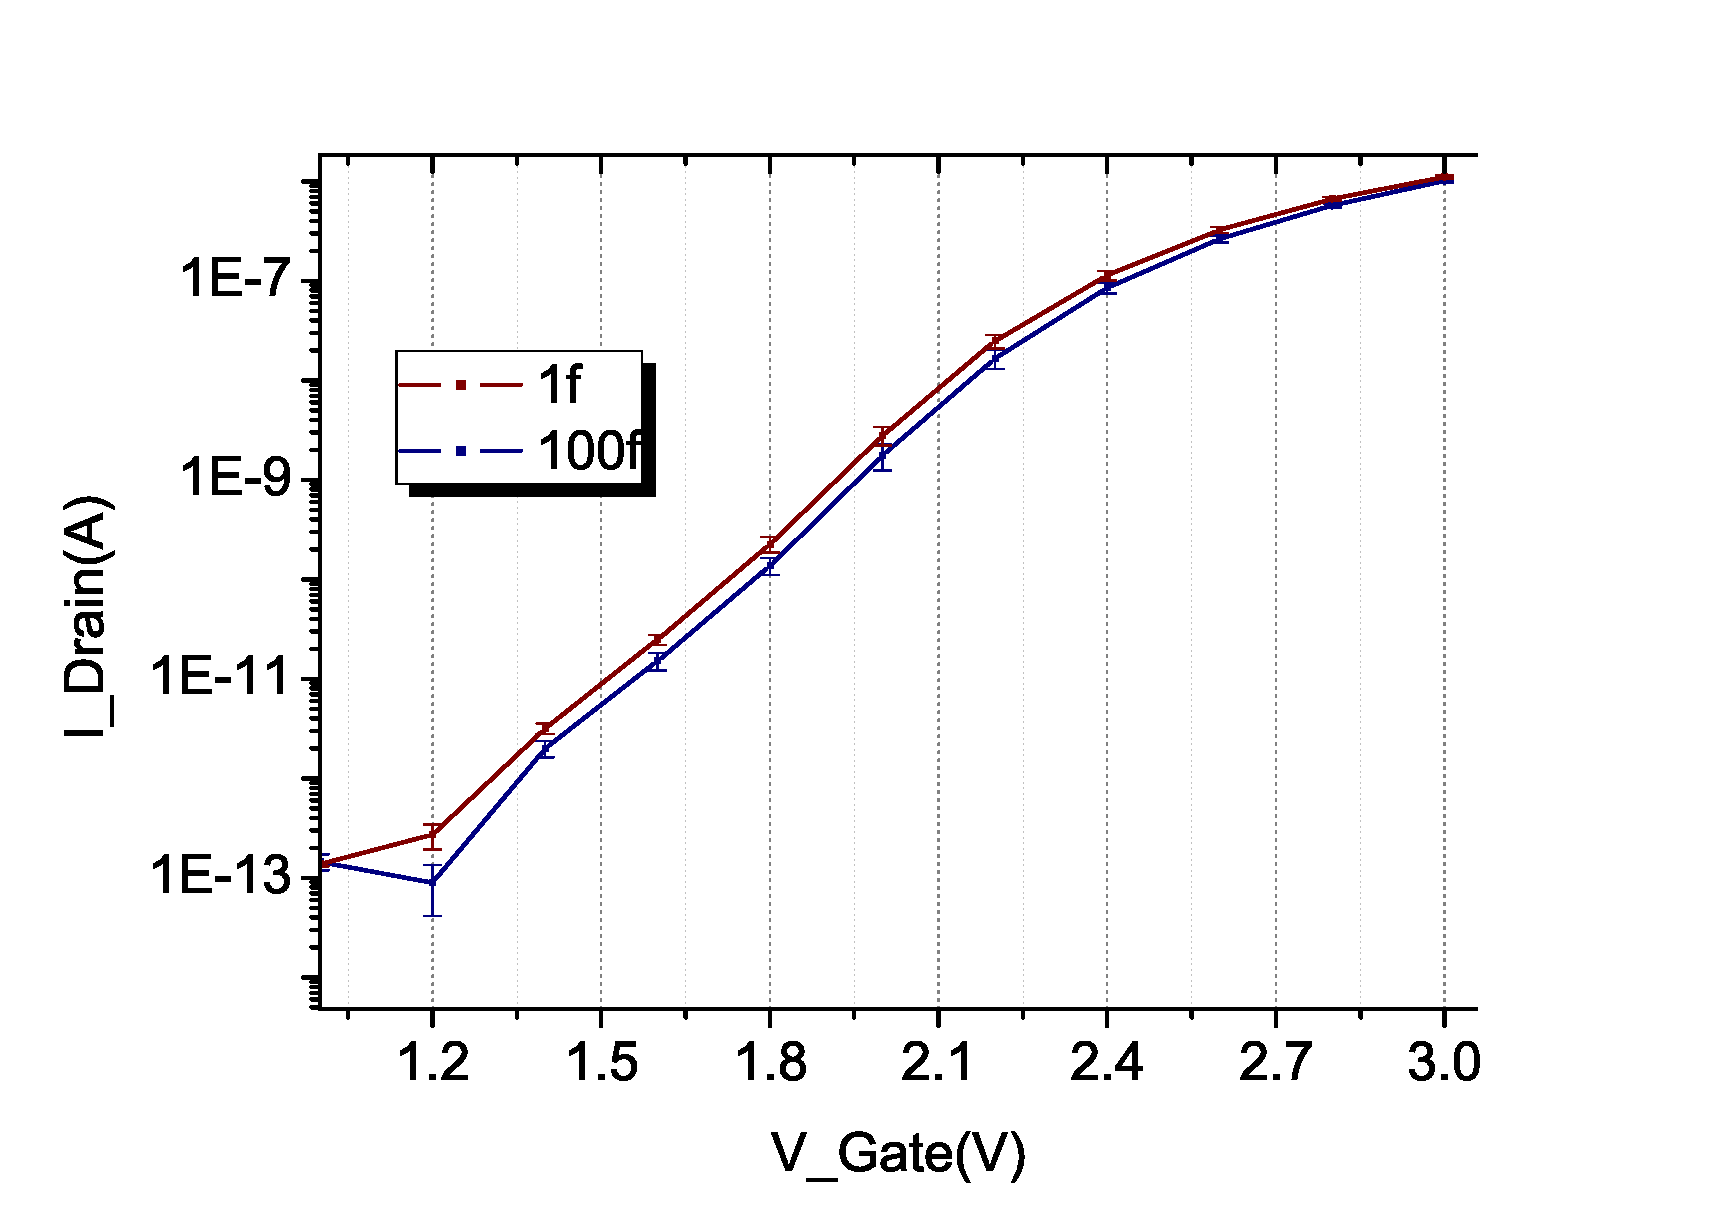
\includegraphics[scale=0.3]{images/chapter3/208_devices/L2-7_log.eps}
            (a)
        \end{minipage}
        \hfill
        \begin{minipage}[t]{0.5\textwidth}
            \raggedleft
            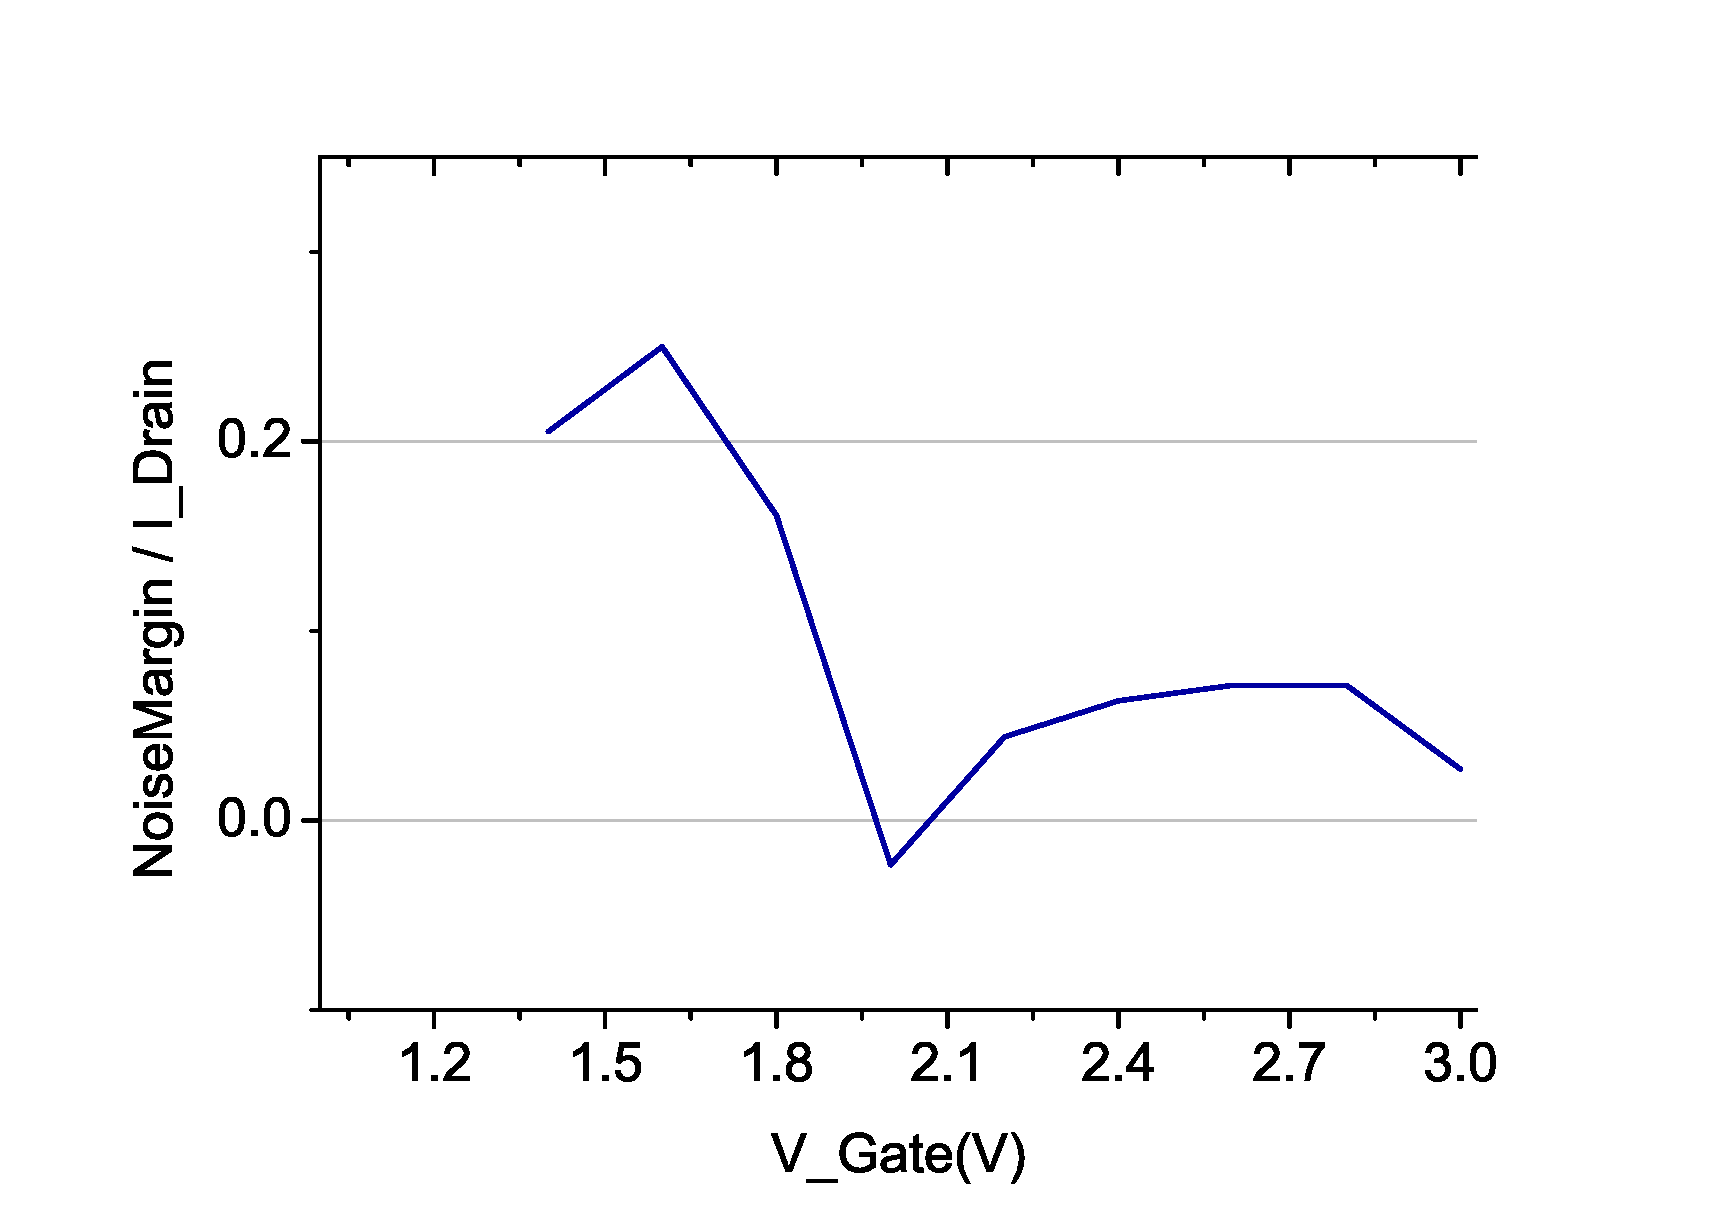
\includegraphics[scale=0.3]{images/chapter3/208_devices/L2-7_margin.eps}
            \centering
            (b)
        \end{minipage}
        \vfill
        \begin{minipage}[t]{0.5\textwidth}
            \centering
            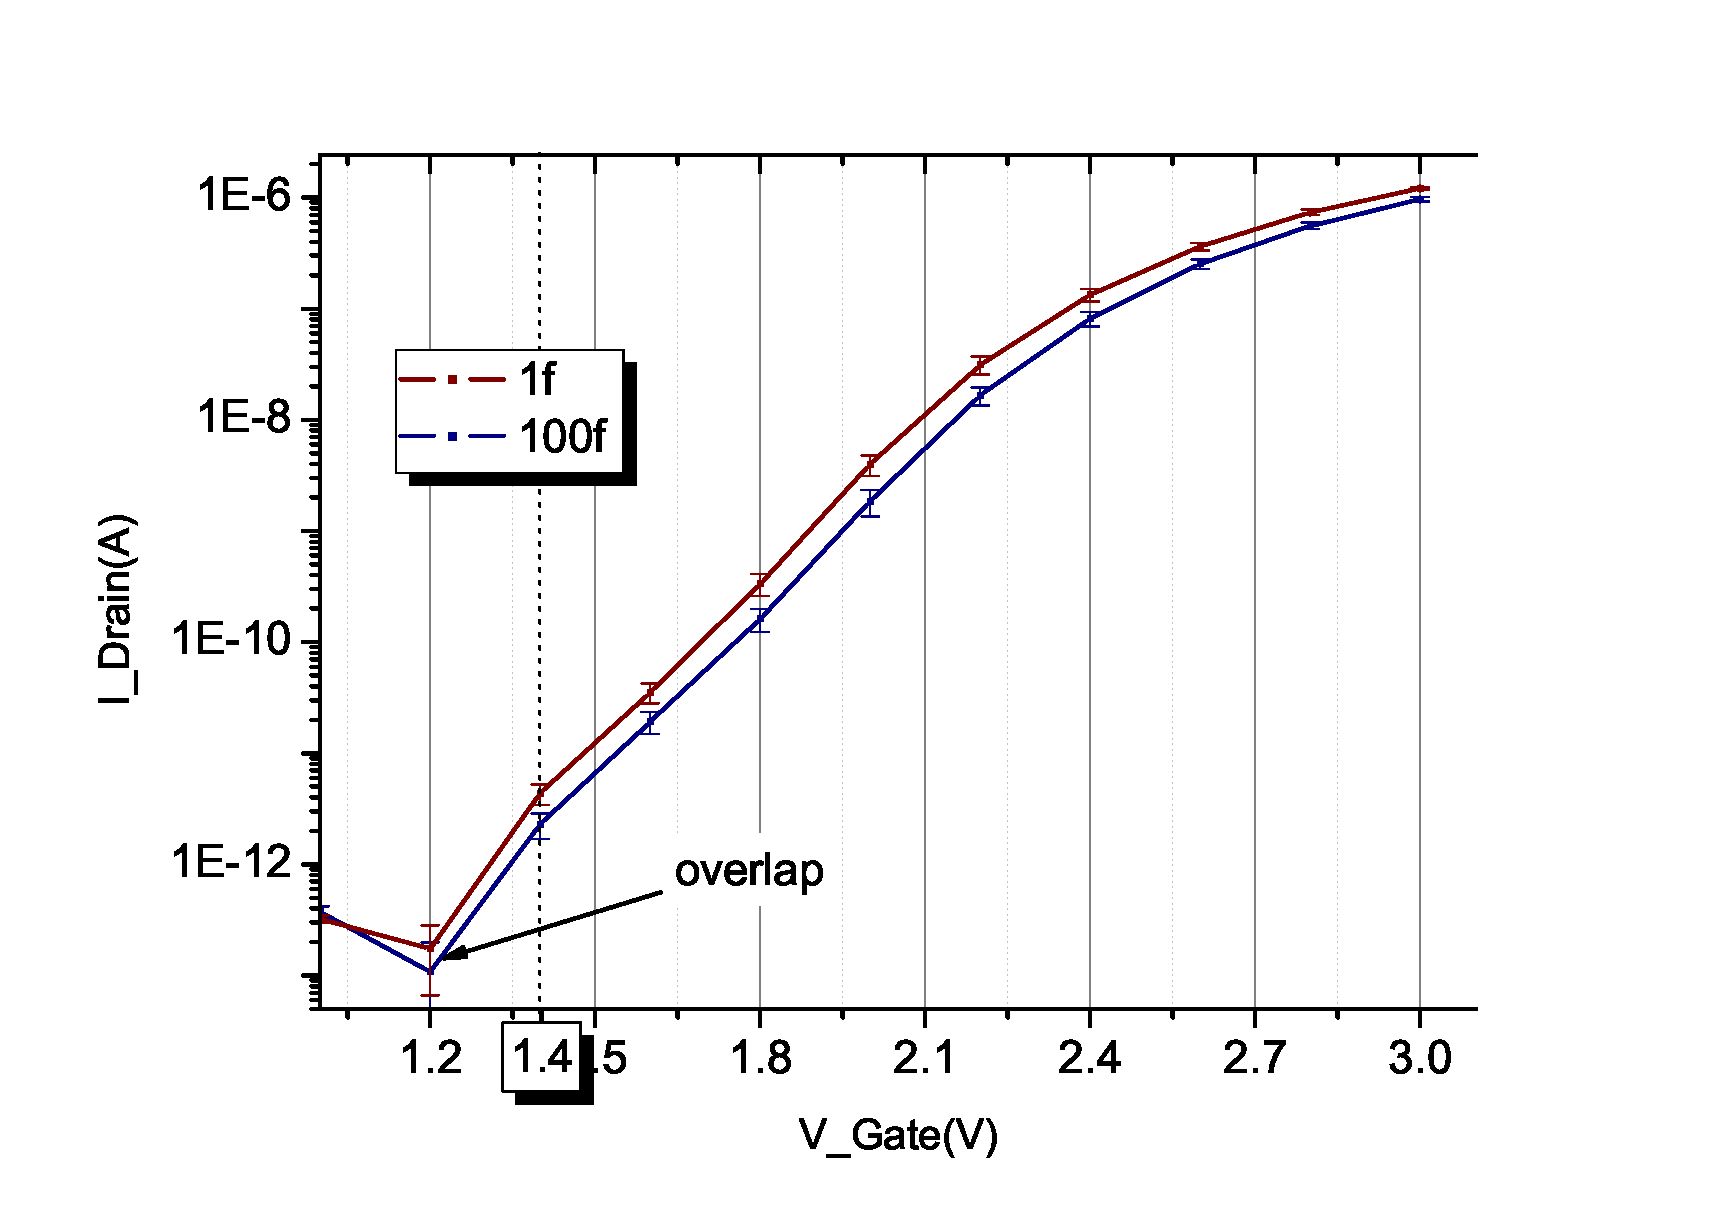
\includegraphics[scale=0.3]{images/chapter3/208_devices/L2-8_log.eps}
            (c)
        \end{minipage}
        \hfill
        \begin{minipage}[t]{0.5\textwidth}
            \raggedleft
            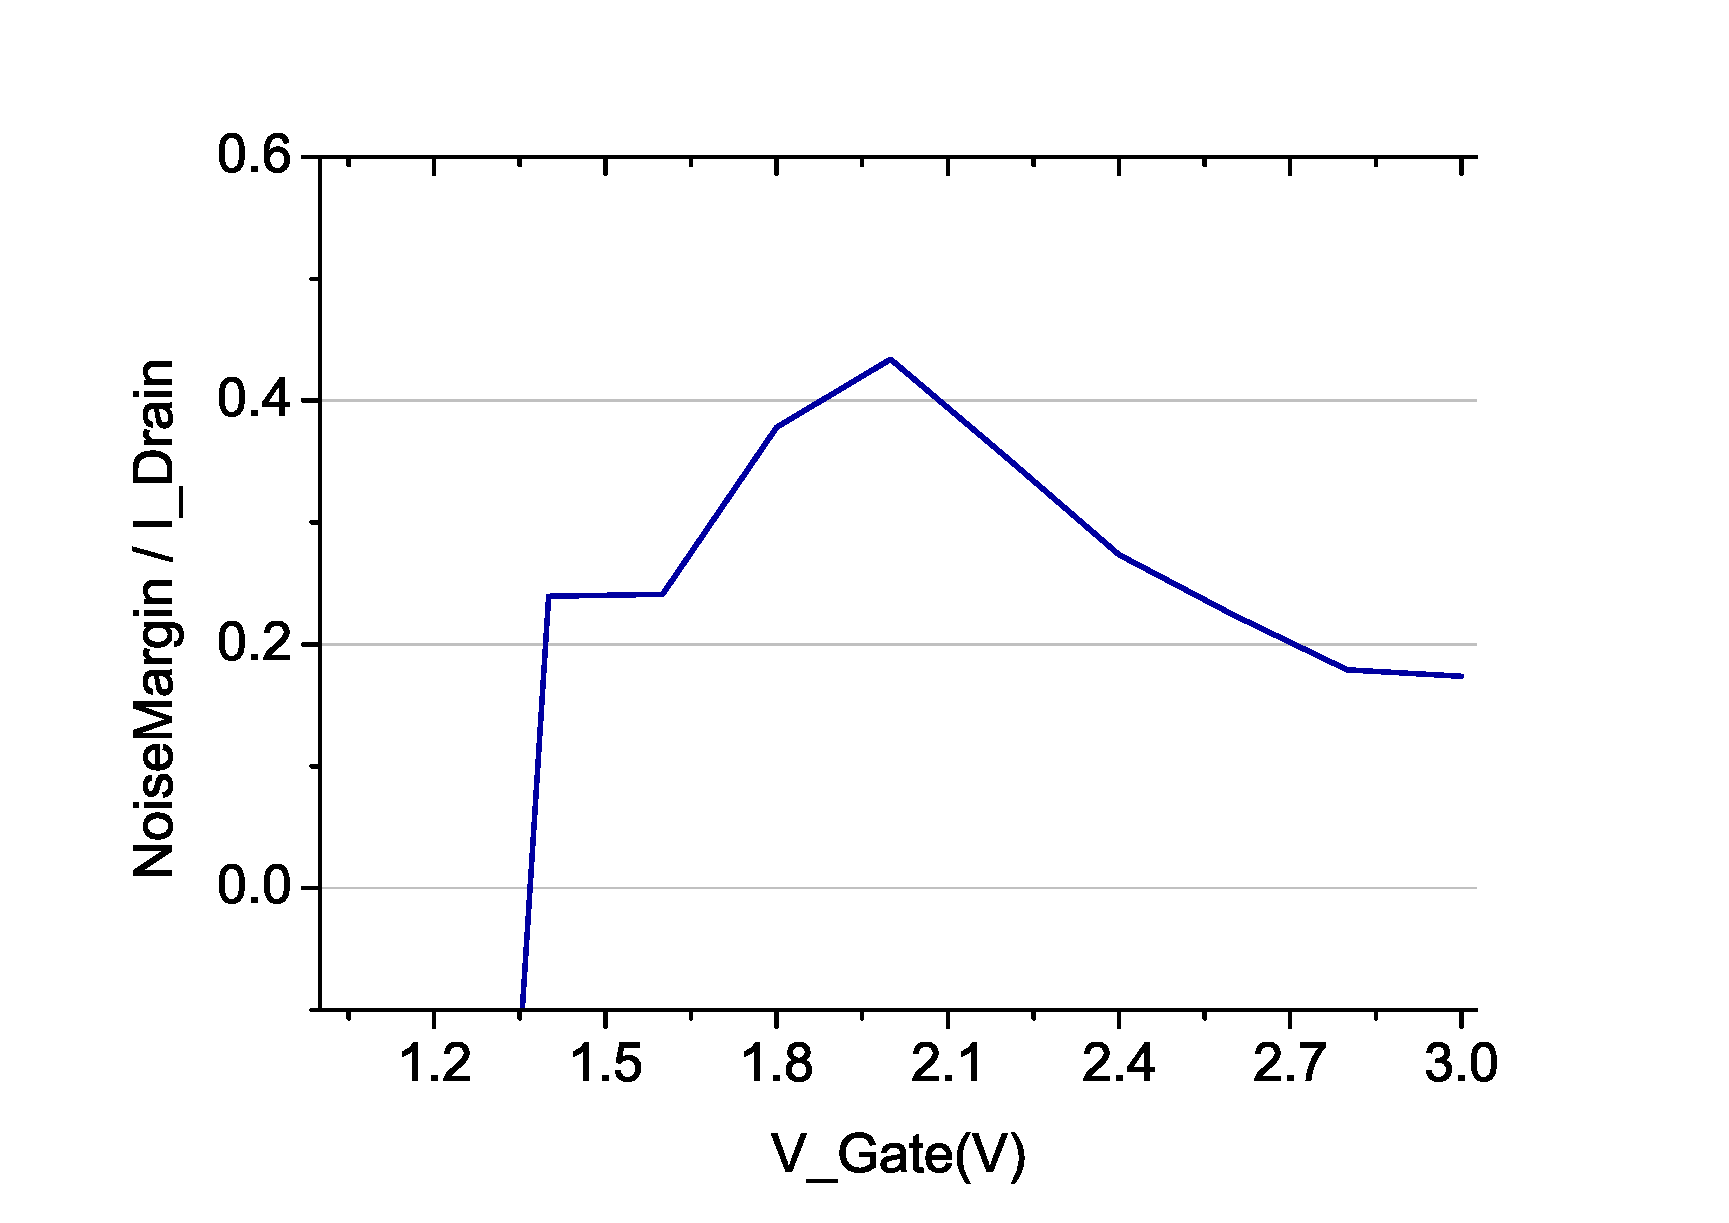
\includegraphics[scale=0.3]{images/chapter3/208_devices/L2-8_margin.eps}
            \centering
            (d)
        \end{minipage}
        \vfill
        \begin{minipage}[t]{0.5\textwidth}
            \centering
            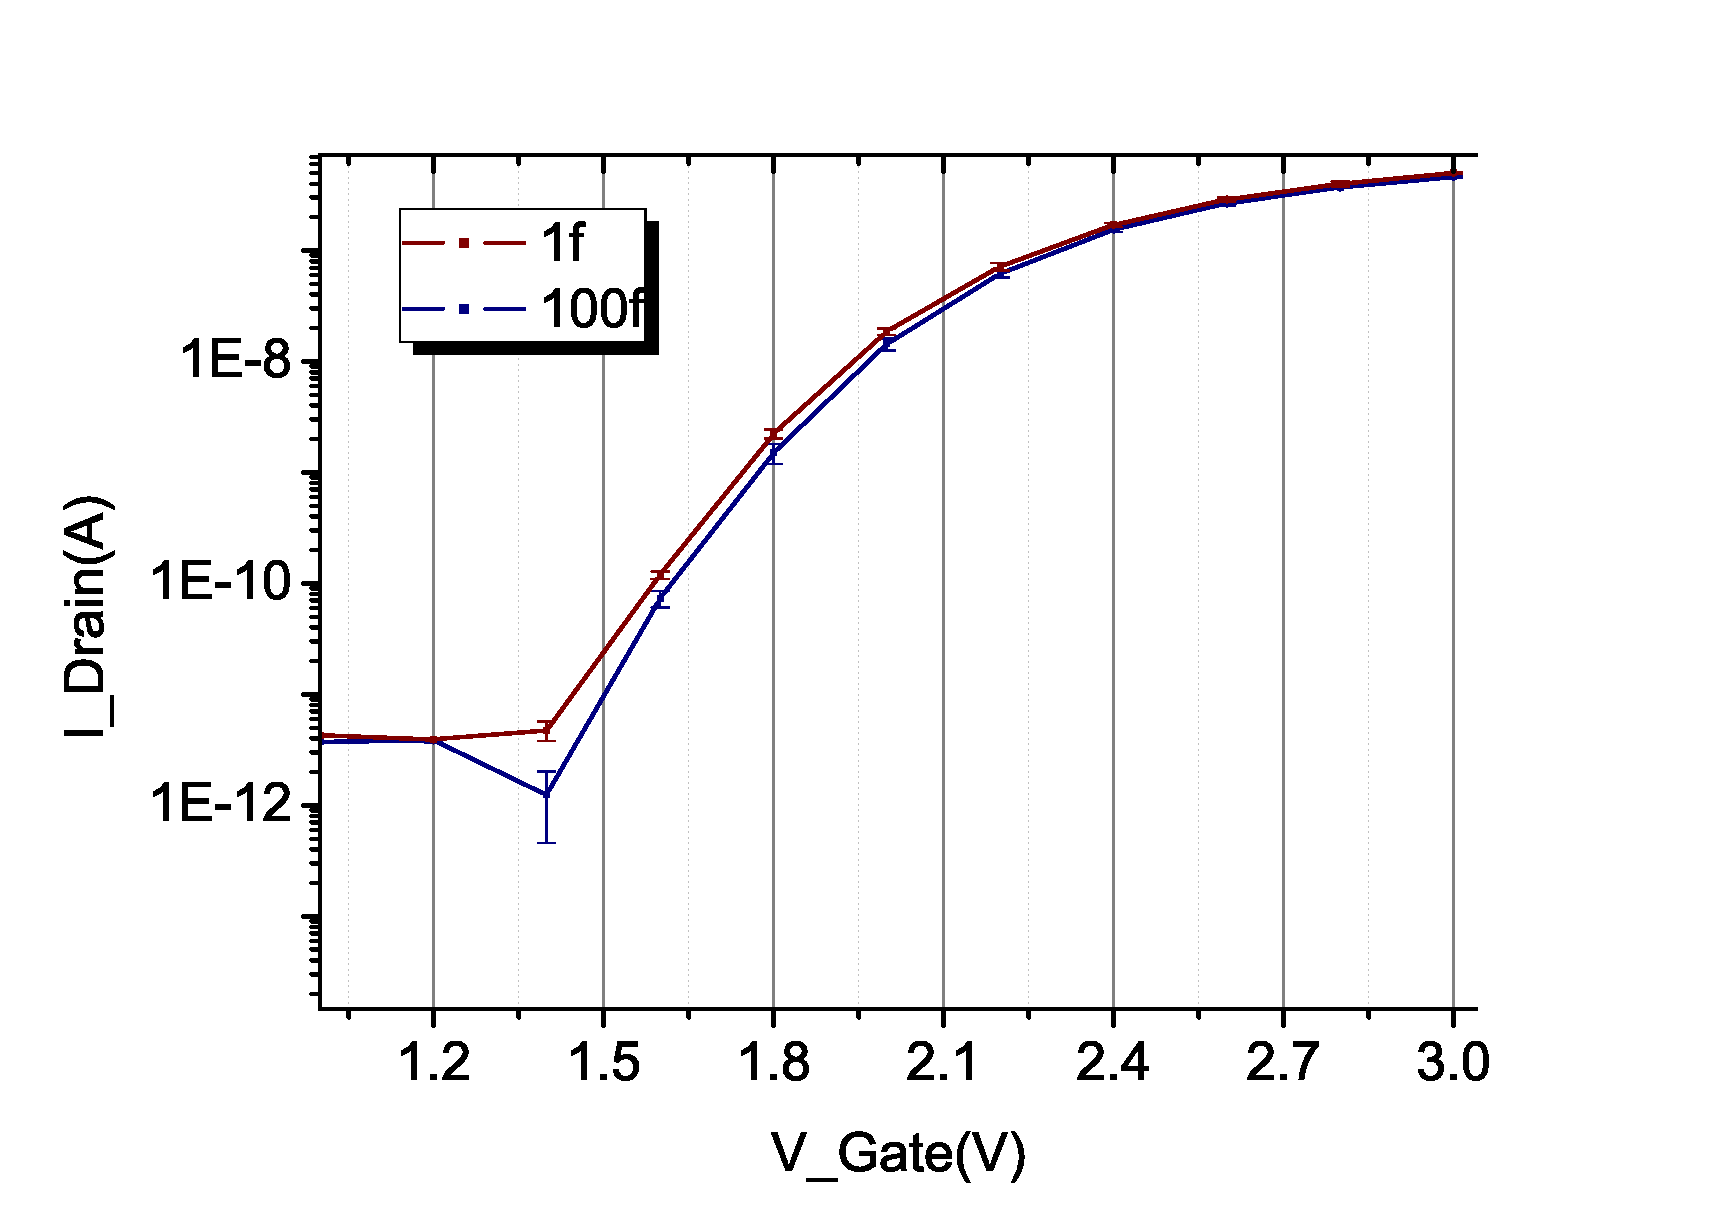
\includegraphics[scale=0.3]{images/chapter3/208_devices/L2-12_log.eps}
            (e)
        \end{minipage}
        \hfill
        \begin{minipage}[t]{0.5\textwidth}
            \raggedleft
            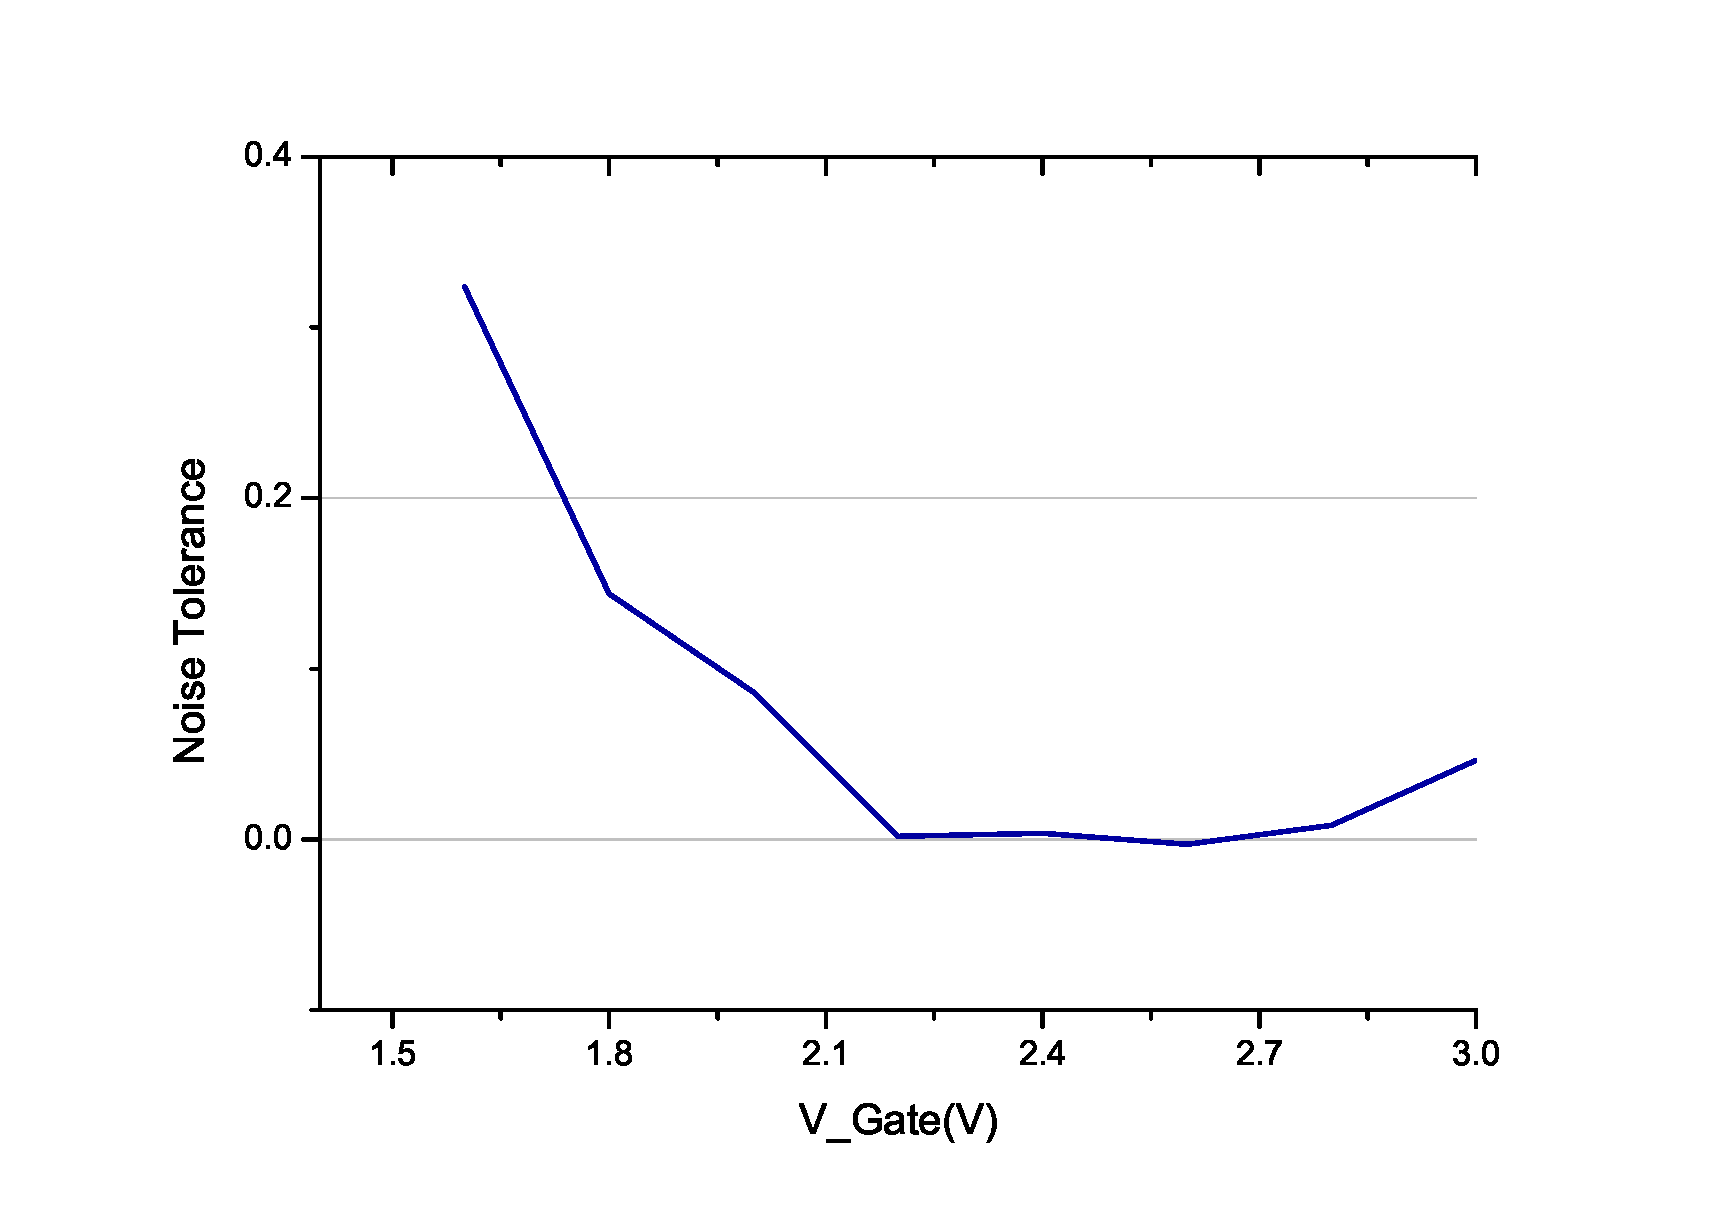
\includegraphics[scale=0.3]{images/chapter3/208_devices/L2-12_margin.eps}
            \centering
            (f)
        \end{minipage}
    \end{minipage}
    \caption{\textbf{(a), (c), (e)} $I_D$-$V_G$ curves for three nanowire devices placed under solution with DNA concentration of 1f and 100f.
                \textbf{(b), (d), (f)} are the noise tolerance of the three devices respectively.}
    \label{fig:SD_Device}
\end{figure}
We present analysis results from three nanowire devices in Fig.\ref{fig:SD_Device}.
Figure (a), (c), (e) are the $I_D$-$V_G$ curves of three devices and Fig.\ref{fig:SD_Device}(b), (d), (f) are the noise tolerance respectively.
One can observe in (b) and (d) that there is first a rising trend then followed by a drop as gate voltage decreases.
The drop does not exist in (f) may because the measurement failed before the drop appears (The failure is because the $I_D$ is too small to be detected.).
But one can still observe the rising trend.
The highest points of (b) and (d) locate in the weak inversion region and is adjacent to the transition region (The region between strong inversion and weak inversion region).
We therefore suggest that it is where nanowire should have better sensitivity.

\subsection{$g_m$-$I_D$ Plot} \label{section:disparityBio}
We plot the $g_m$-$I_D$ curves for the data in Fig.\ref{fig:SD_allT}.
The result in Fig.\ref{fig:gmId} clearly proves our two assumptions for dealing with the device variability problem, which we have discussed in section.\ref{sec:assumpDiscuss}.

\begin{figure}[htb]
    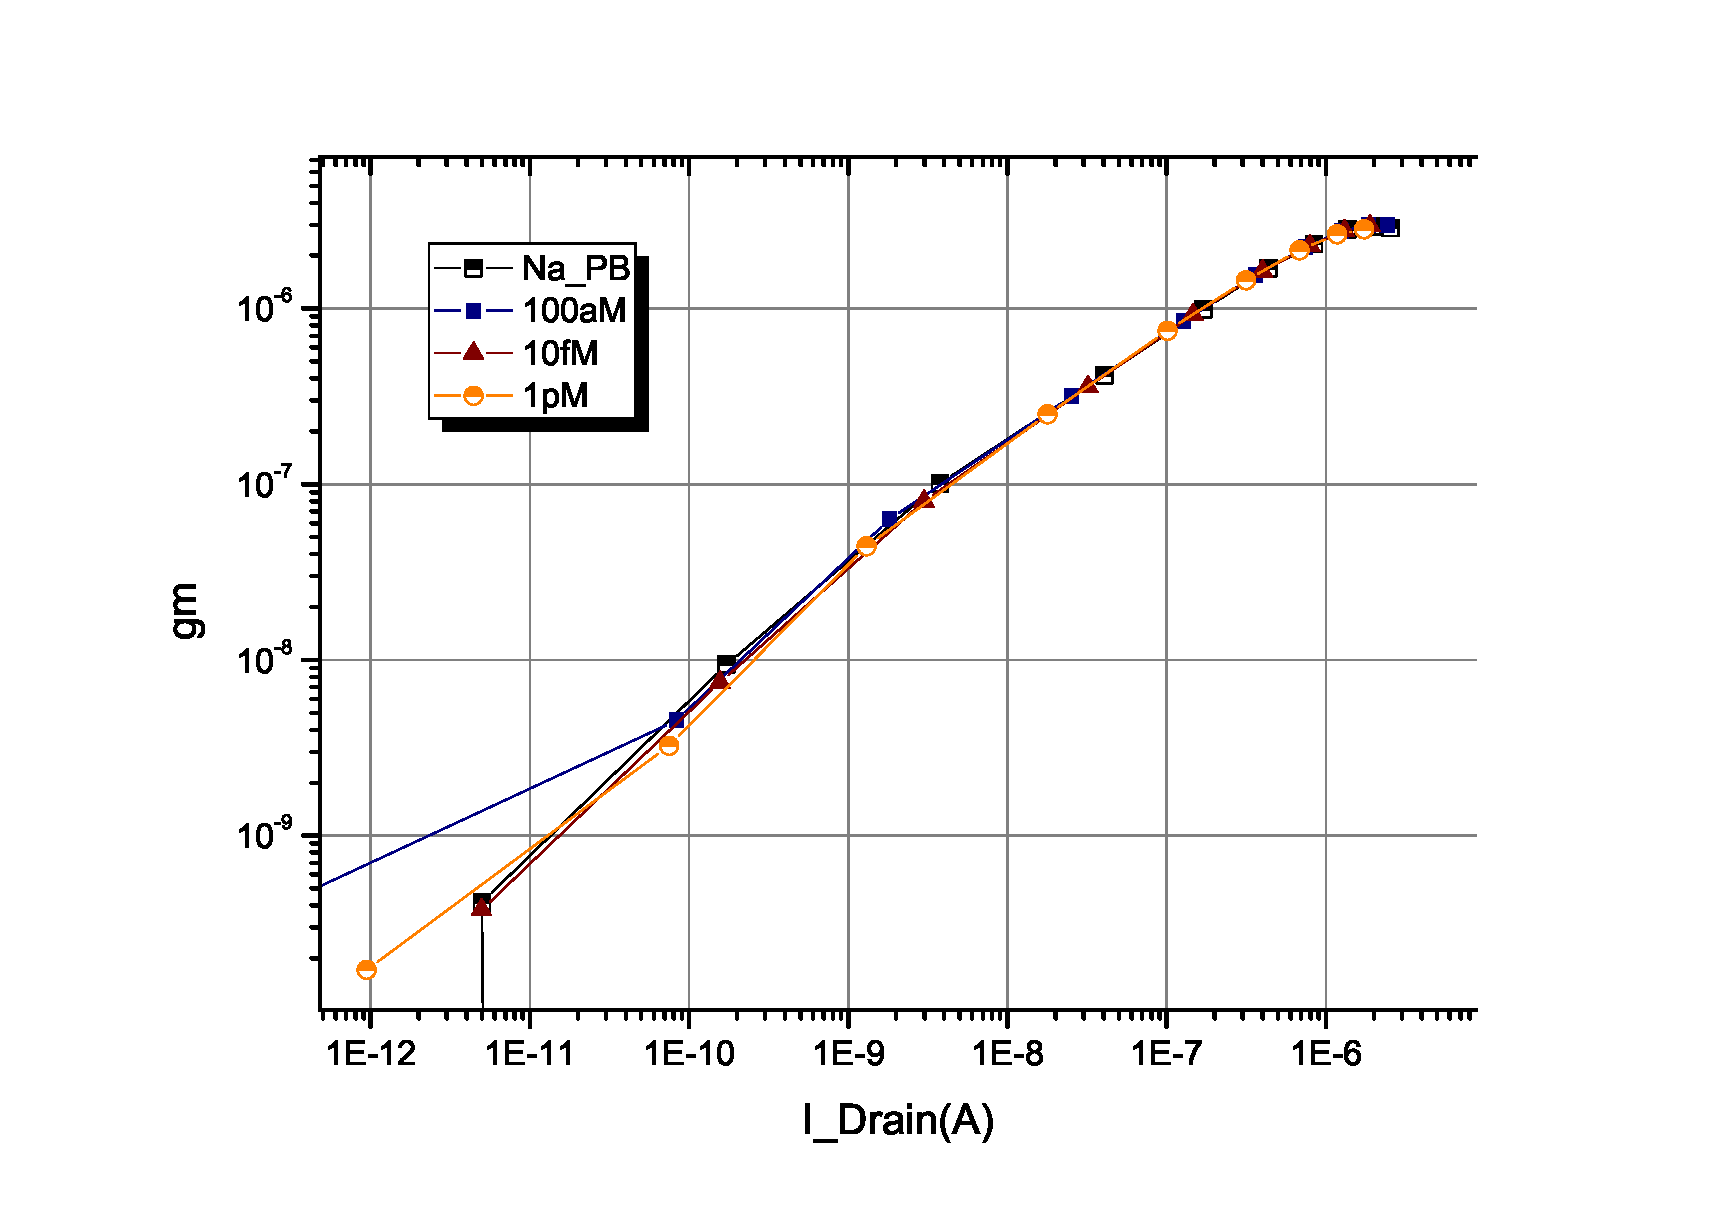
\includegraphics[width=1\textwidth]{images/chapter3/Id_Dev_bio.eps}
    \caption{The $g_m$-$I_D$ curve obtained by the $I_D$-$V_G$ curve in Fig.\ref{fig:SD_allT}. The curves start splitting after $I_D$ > 1$\mu$A where the device may enter into strong inversion region.}
    \label{fig:gmId}
\end{figure}

In Fig.\ref{fig:gmId}, the $g_m$ of nanowire is almost independent of concentration and merely depends on $I_D$ when $I_D$ ranges from 0.1nA to 1$\mu$A.
In fact, the curves start splitting after $I_D$ > 1$\mu$A.
It means the device is no longer in weak inversion region but enters strong inversion region.

With the data from Fig.\ref{fig:SD_allT}, we may find the equivalent voltage change induced by the concentration difference based on the assumption 2 (section.\ref{sec:assumpDiscuss}).
The values is changeable, which may depend on the gate-coupling coefficient (Eq.\ref{eq:Ikappa}).
\begin{table}[tbh]
    {\fontfamily{}\fontsize{10}{14}\selectfont
    \centering
    \begin{tabular}{l|c|c|c}
        Concentration Difference & Na\_PB - 100aM & 100aM - 10fM & 10fM - 1pM \\
        \hline
        Equivalent voltage value & $30mV - 40mV$ & $200mV - 280mV$ & $38mV - 60mV$ \\
    \end{tabular}
    \caption{The equivalent voltage value generated by the concentration difference. They are obtained by the data from Fig.\ref{fig:gmId}. The $I_D$ difference of different concentration is divided by their $g_m$ ($\Delta I_D = g_m\Delta V_G$).}
    \label{tb:CdV}
    }
\end{table}










\section{Electrical Measurements}
This section presents the data analysis results.
The data are obtained from our measurements with the source meter (Keithley 2602).
To exclude the effect of ions, we placed nanowire devices in the distilled deionized water instead of biomolecule solution.
And there is no DNA probe on the surfaces of poly-silicon channel.

\subsection{Front Gate and Back Gate}
Our nanowire has two gates available: floating gate (liquid gate) and back-gate.
We choose floating gate as the operation gate mainly because the floating gate can induce a larger drain current.
In other words, it has higher transconductance (Fig.\ref{fig:IdVgandgbsId}).
In our circuit design, nanowire is placed in a feedback loop where its transconductance is proportional to the loop gain (chapter 5).

\begin{figure}[tbp]
    \centering
    \begin{minipage}[t]{1\textwidth}
        \centering
        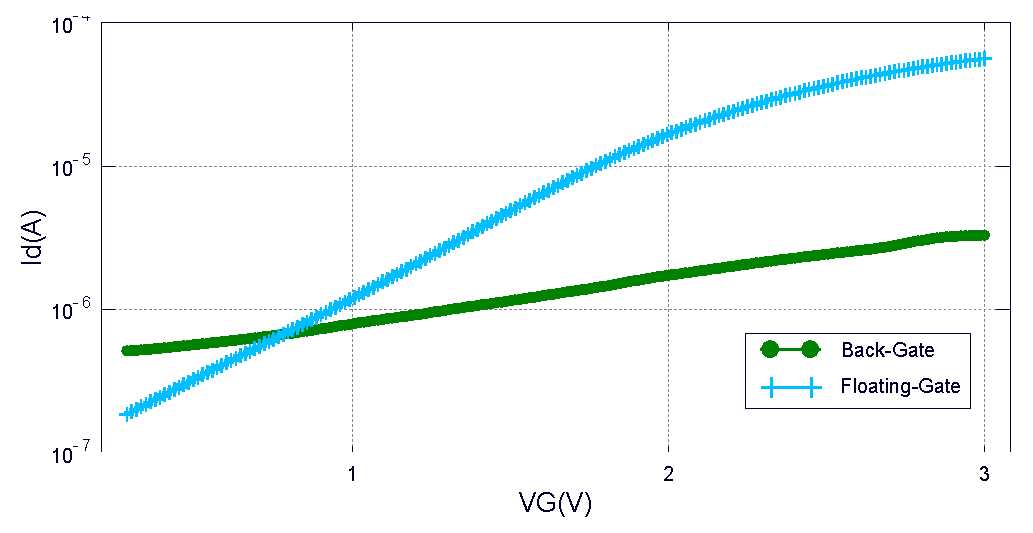
\includegraphics[width=1\textwidth]{images/chapter3/FgBg_Compare_Id.eps}
        \raggedleft
        (a)
    \end{minipage}
    \vfill
    \begin{minipage}[t]{1\textwidth}
        \centering
        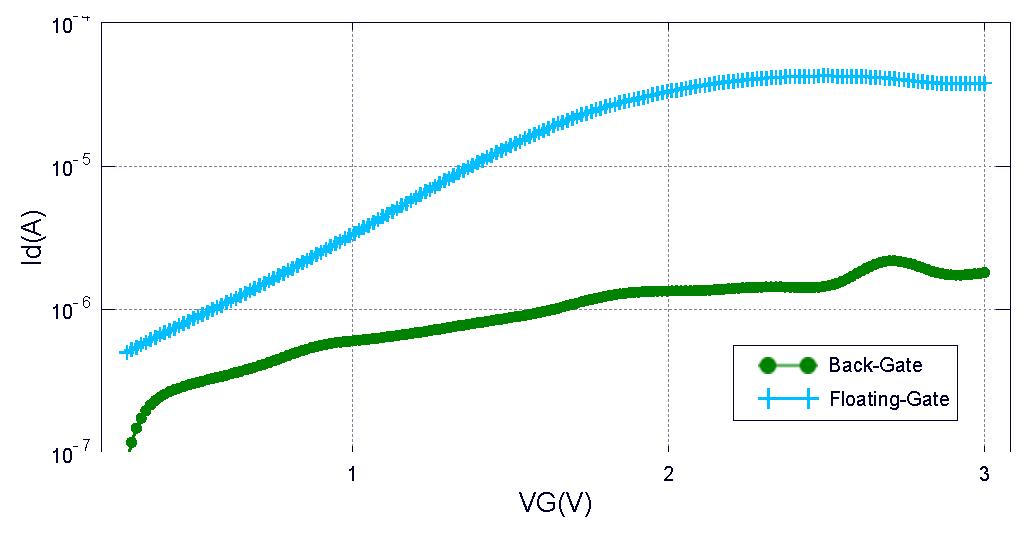
\includegraphics[width=1\textwidth]{images/chapter3/FgBg_Compare_Id_dev.eps}
        \raggedleft
        (b)
    \end{minipage}
    \caption{Comparison between the DC sweep of voltage on the floating gate and back gate. \textbf{(a)} $I_D$. \textbf{(b)} Transconductance ($g_m$). The $I_D$ and $gm$ of the floating gate are larger than the back gate.}
    \label{fig:IdVgandgbsId}
\end{figure}


There are some advantages of back-gate.
One of them is the ability to lower the 1/f noise \cite{C7, C8}.
But this only holds for a very high gate voltage, which is not practical in the integrated circuit design.

\subsection{Transconductance}
The most crucial parameter for our circuit design is the transconductance ($g_m$).
It is acquired by calculating the partial derivative of $I_D$ with respect to $V_{G}$.
Since in section.\ref{section:IdGm} we proved that $g_m$ is dependent on $I_D$, we plot the $g_m$-$I_D$ curve to reveal their relation (Fig.\ref{fig:pIdVg}(b)).

\begin{figure}[!htbp]
    \centering
    \begin{minipage}[t]{1\textwidth}
        \centering
        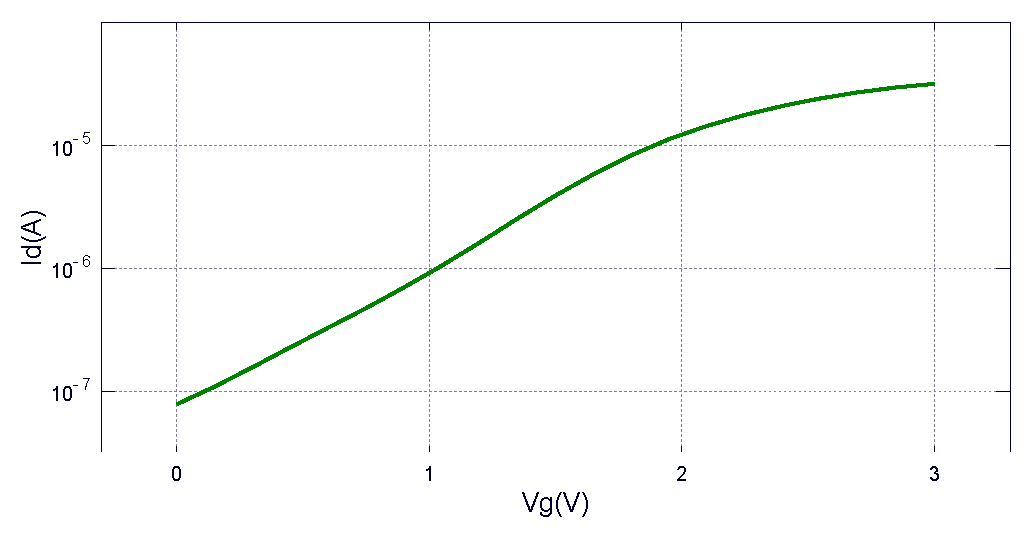
\includegraphics[width=1\textwidth]{images/chapter3/pIdVg.eps}
        \raggedright
        (a)
    \end{minipage}
    \hfill
    \begin{minipage}[t]{1\textwidth}
        \centering
        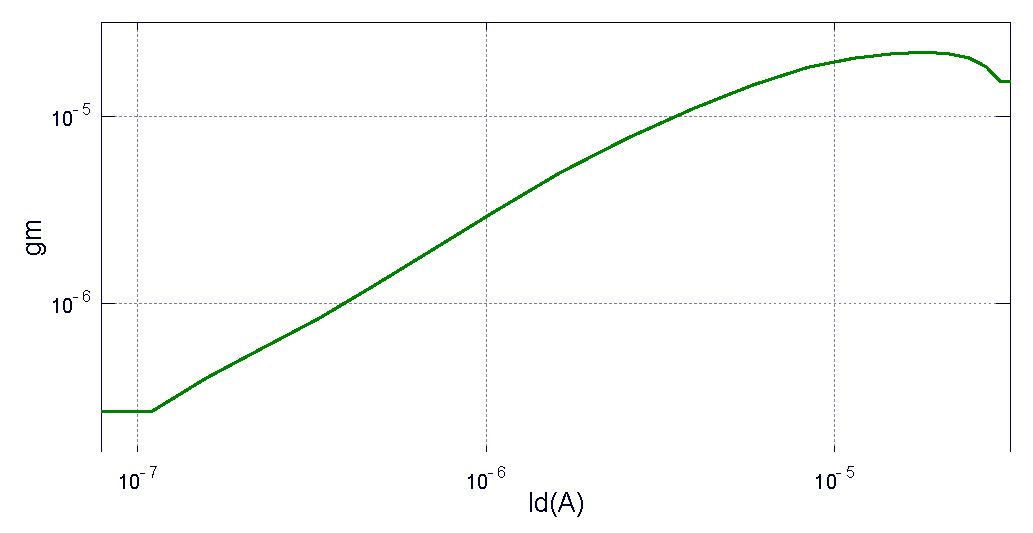
\includegraphics[width=1\textwidth]{images/chapter3/pIdgbs.eps}
        \raggedright
        (b)
    \end{minipage}
    \caption{Eelectrical response of a nanowire device. \textbf{(a)} Sweep $V_G$ and measure the $I_D$ changes. By finding $g_m (\frac{\partial I_D}{\partial V_G}$), \textbf{(b)} the $g_m$-$I_D$ curve is plotted.}
    \label{fig:pIdVg}
\end{figure}

The $g_m$-$I_D$ plot indicates that there is a ``linear region'' where $g_m$ is proportional to $I_D$.
This corresponds to our derivation in Eq.(\ref{eq:gm_weak}).
It can be can recognize that our nanowire device is operated in weak inversion region when $I_D$ is less than 10$\mu$A.
Therefore, by the section.\ref{section:biasVg}, we decide the $I_D$ of our nanowire should be operated below 10$\mu$A.

We also proved that the transconductance under this region is unaffected by $V_{DS}$.

\begin{figure}[tbp]
    \centering
    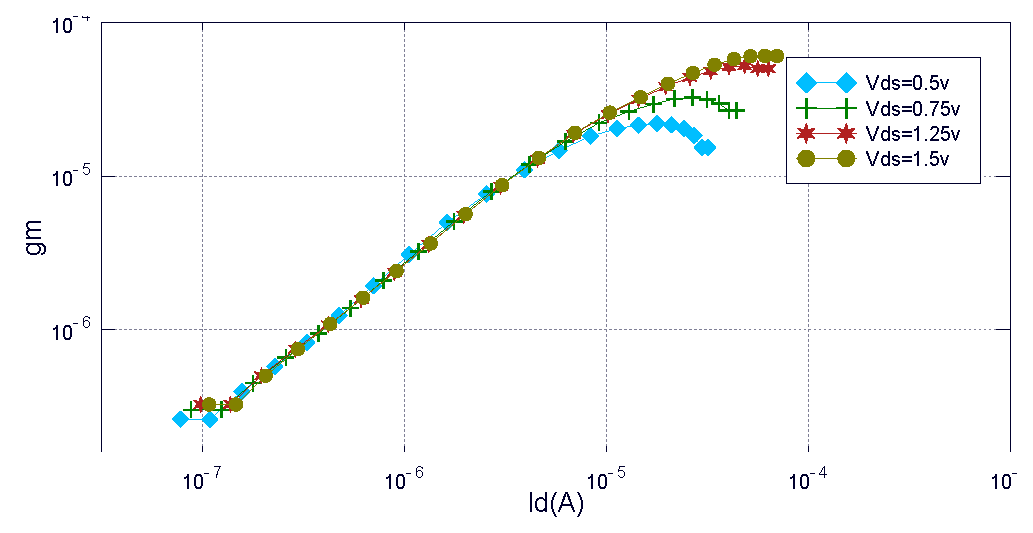
\includegraphics[width=1\textwidth]{images/chapter3/pIdgbs_Vd.eps}
    \caption{$gm$-$I_D curves$ with $V_{DS}$ variance}
    \label{fig:Idgbs_Vd}
\end{figure}

\subsection{Drain-to-source impedance ($r_{ds}$)} \label{sec:ch3rds}
In our circuit design, $V_{DS}$ is kept constant.
According to the measurement data from Fig.\ref{fig:Idgbs_Vd}, $V_{DS}$ of 0.7V is enough to keep nanowire in saturation region for $V_G$ ranging from 0v to 3v.

We concern about how $I_D$ effect $r_{ds}$.
The way we obtained $r_{ds}$ is as follows:
\begin{enumerate}
    \item Perform $I_D$-$V_G$ sweep with two different $V_D$. We picked $V_D$ values of 0.75V and 1V.
    \item Find the difference of $I_D$ at each $V_G$ biasing point and divide it by the difference of $V_D$.
\end{enumerate}
The result is presented in Fig.\ref{fig:rds}.
It shows that the $r_{ds}$ is inversely proportional to $I_D$.
Its value ranges from $40k \Omega$ to $30M \Omega$.
This result becomes useful when we perform the analysis of impedance matching in chapter 5.


\begin{figure}[tbp]
    \centering
    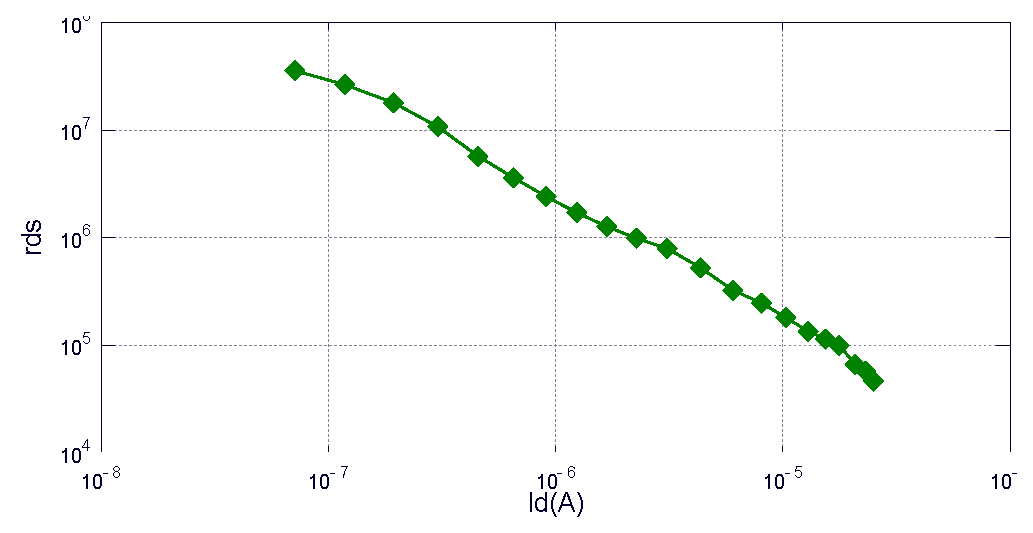
\includegraphics[width=1\textwidth]{images/chapter3/rds_I.eps}
    \caption{$I_D$-$r_{ds}$ plot}
    \label{fig:rds}
\end{figure}


\subsection{Device variability Problem exists}
We measured two nanowire devices which lie on the same wafer and are immersed with the same testing PBS solution.
Below, the $g_m$-$I_D$ plot (Fig.\ref{fig:disparity}) shows that even the environment is same, two devices exhibit different electrical responses.
\emphy{This problem causes issues such as non-uniform specification for measurement or bad quality assurance in a mass production.
We try to diminish it by performing the variability-resisting measurement, which have been mentioned in chapter 1.}

\begin{figure}[!htb]
    \centering
    \def\svgwidth{width=0.67\textwidth}
    % \fontsize{5}{15}\selectfont
    % \input {images/chapter3/pDisparity.pdf}
    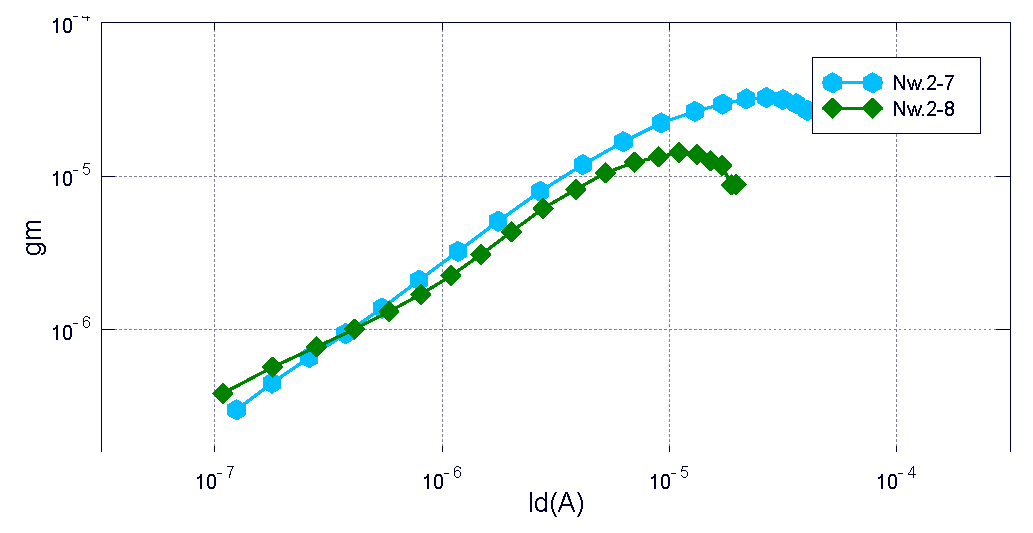
\includegraphics[width=1\textwidth] {images/chapter3/pDisparity.eps}
    \caption{Device variability problem cause nanowire devices with same environment can exhibit different electrical responses.}
    \label{fig:disparity}
\end{figure}


\section{Conclusion and Design Specification} \label{sec:spec3}

Table.\ref{tb:NWcharacter} summarizes the electrical characteristics of our nanowire.
\begin{table}[h!bp]
    {\fontfamily{}\fontsize{10}{14}\selectfont
    \centering
    \begin{tabular}{c|c|c|c|c}
        Operation Region & $I_D$ & $V_G$ & $g_m$ & $r_{ds}$ \\
        \hline
        Cut off & $< 100n A$ & $< 0 V$ & - & - \\
        weak inversion & $100n A$ - $10\mu A$ & $0 V$ - $2.5V$ & $200n $ - $20\mu$ & $50M\Omega$ - $200k\Omega$ \\
        strong inversion & $> 1\mu A$ & $> 2.2V$ & $20\mu$ - $30\mu$ & $< 200k\Omega $ \\
    \end{tabular}
    \caption{Electrical characteristics. There are overlaps due to the device variability}
    \label{tb:NWcharacter}
    }
\end{table}

We hence decide the design specification for DC-sweep mode as Table.\ref{tb:DCspec}.
\begin{table}[!htbp]
    {\fontfamily{}\fontsize{10}{14}\selectfont
    \centering
    \begin{tabular}{c|c|c}
        $I_D$ & $g_m$ & $V_G$\\
        \hline
        $100n A$ - $30\mu A$ & $200n $ - $20\mu$ & $0.5V$ - $3V$\\
    \end{tabular}
    \caption{Specification for DC-sweep mode}
    \label{tb:DCspec}
    }
\end{table}


\emphy{As for Transient Measurement mode, section.\ref{section:biasVg} suggests that the device should be operated in the weak inversion region adjacent to the strong inversion region.
And Table.\ref{tb:CdV} indicates that the voltage change ($\Delta V_G$) induced by concentration difference ranges from $20mV$ to $280mV$.
These factors give result to the table of device characteristics for transient measurement (Table.\ref{tb:ACinput}).}

\emphy{The design specification for Transient Measurement mode is presented in Table.\ref{tb:ACSpec}.
$\Delta I_D$ is the multiplication of $\Delta V_G$ and $g_m$ from Table.\ref{tb:ACinput}.
The limitation of input referred noise (referred to the gate) is 10\% of the minimal $\Delta V_G$ ($20m V \times 10\% 2mV$) or 10\% of the minimal $\Delta I_D$ ($1\mu \times 20mV \times 10\%= 2n A$) .
The transimpedance (input current to output voltage) is $5M \Omega$.
This is because the minimal $\Delta I_D$  is $20n A$ and a transimpedance of $5M \Omega$ allows the output voltage to be larger than $0.1 V$.
The bandwidth is $1k$ Hz.
The input signal $\Delta I_D$ is a very slow signal with the speed less than $10$ Hz.
However, we implement a modulation method in chapter 5, which resembles the method adopted by \cite{Jlockin}.
The input signal is modulated to a higher frequency to avoid the low frequency noise.
Thus, we determined that the bandwidth of the circuit should be at least $1k$ Hz.
}

\begin{table}[!htbp]
    {\fontfamily{}\fontsize{10}{14}\selectfont
    \centering
    \begin{tabular}{c|c|c}
        $I_D$ & $g_m$ & $\Delta V_G$ \\
        \hline
        $600n A$ - $10\mu A$ & $1\mu $ - $20\mu$ & $20mV$ - $280mV$\\
    \end{tabular}
    \caption{The summation of the nanowire characteristics when applied with Transient Measurement mode circuit}
    \label{tb:ACinput}
    }
\end{table}

\begin{table}[!htbp]
    {\fontfamily{}\fontsize{10}{14}\selectfont
    \centering
    \begin{tabular}{c|c|c|c|c}
        $\Delta I_D$&Input Referred Noise&Input Referred Noise&Transimpedance Gain &Bandwidth\\
                   & (referred to $V_G$)& (referred to $I_D$)  & (max) & \\
        \hline
        $20n A$ - $2.8\mu A$&$< 2m V$& $< 2n A$&$5E6(\frac{V}{A})$&$> 1k$ (Hz)\\
    \end{tabular}
    \caption{Specification for Transient Measurement mode circuit}
    \label{tb:ACSpec}
    }
\end{table}





 

